
In this subsection, a wildfire dataset is used to compare the drought impact database with reported wildfire occurrences.

\subsection{Exploratory Data Analysis}

\begin{figure}[htbp]
\centering
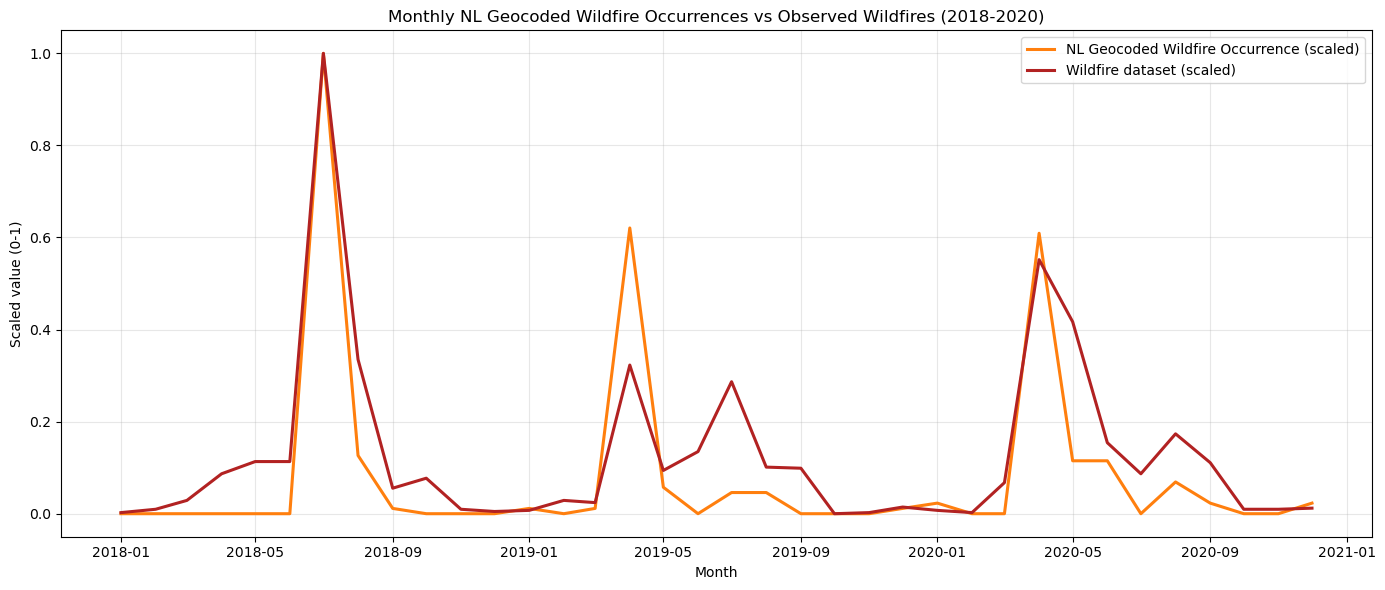
\includegraphics[width=0.95\textwidth]{figures/Monthly NL Geocoded Wildfire Occurrences vs Observed Wildfires (2018-2020).png}
\caption{Monthly normalized NL-geocoded wildfire occurrences compared with observed reference wildfires from 2018 to 2020.}
\label{fig:fires}
\end{figure}

As an initial evaluation, the wildfire events extracted by the LLM were compared with a separate wildfire reference dataset for the Netherlands. The reference dataset contains fire department call records and therefore represents reported wildfire occurrences rather than the size or severity of the fires. Monthly wildfire counts from both datasets were compared between January 2018 and December 2020.

Because both datasets use different scales, the two time series were separately transformed using min--max normalization to values between $[0,1]$. This allows comparison of changes over time rather than differences in the absolute number of events.

As shown in Figure~\ref{fig:fires}, both datasets show similar seasonal patterns, with a clear peak during the summer of 2018. The LLM-extracted wildfire series captures most peaks observed in the reference dataset during the following summers. However, a clear difference occurs in July 2019, where the reference dataset shows a strong increase in wildfire occurrences that is not visible in the extracted dataset. This period is therefore investigated further in the case study analysis. Overall, both datasets show similar temporal patterns after normalization.


\subsection{Case Study Analysis}

Based on the exploratory analysis, three periods were selected for further investigation: the major wildfire peak of July 2018, the smaller wildfire peak of April 2019, and the missing wildfire peak of July 2019. These periods show examples where the extraction framework successfully captures wildfire activity and where differences between datasets occur.

The extracted wildfire events were compared with the reference wildfire dataset at a monthly level. For this analysis, the recency window was set to 0, meaning that only impacts classified as ongoing or occurring within the previous month were included. Only wildfire occurrence events were considered, while wildfire risk indicators were excluded to evaluate how well the framework captures actual wildfire events.

\paragraph{July 2018}

Figure~\ref{fig:wildfire-geocoding-comparison-jul2018} compares observed wildfire occurrences with wildfire events extracted from newspaper articles during July 2018. The point-level representation shows that extracted locations do not always exactly match the recorded wildfire locations. This is expected because newspapers often report municipalities, nature areas, or larger regions instead of exact coordinates.
\begin{figure}[!htbp]
\centering
\begin{subfigure}[t]{0.49\textwidth}
\centering
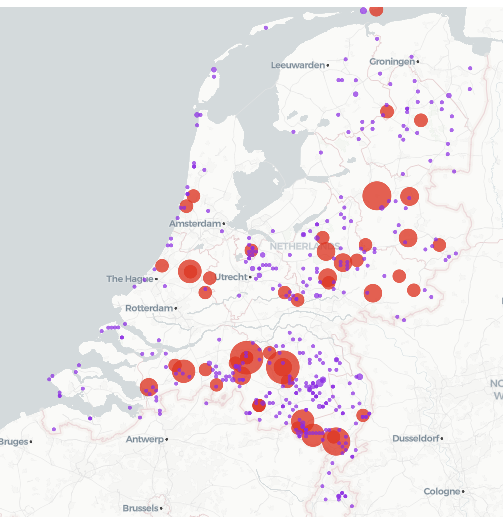
\includegraphics[width=\textwidth]{figures/Wildfires-Jul-2018-point.png}
\caption{Point-level geocoding results.}
\label{fig:wildfire-point-jul2018}
\end{subfigure}
\hfill
\begin{subfigure}[t]{0.49\textwidth}
\centering
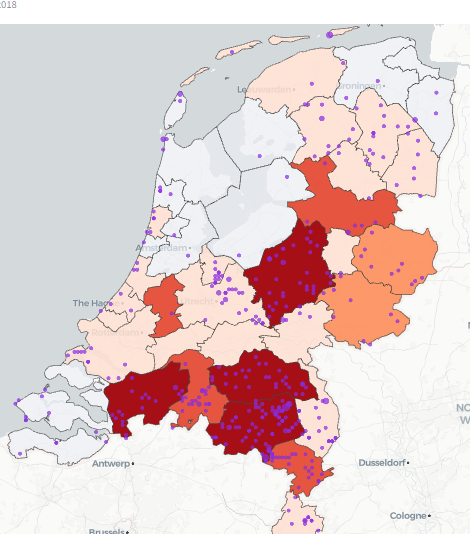
\includegraphics[width=\textwidth]{figures/Wildfires-Jul-2018-Nuts.png}
\caption{NUTS-3 aggregated geocoding results.}
\label{fig:wildfire-nuts-jul2018}
\end{subfigure}
\caption{Comparison of wildfire event locations extracted from news articles for July 2018 using point-level geocoding and NUTS-3 aggregation.}
\label{fig:wildfire-geocoding-comparison-jul2018}
\end{figure}

Despite these differences, most extracted locations are close to areas with recorded wildfire activity. This suggests that the extracted events generally correspond to real wildfire occurrences. After aggregation to the NUTS-3 level, regional wildfire patterns become easier to interpret. In particular, the higher wildfire concentrations in the southern Netherlands, especially North Brabant and surrounding regions, are captured reasonably well. 

The comparison also shows regions where fewer events are extracted compared with the reference dataset. For example, wildfire activity around Utrecht appears stronger in the reference dataset than in the newspaper-derived dataset. Possible explanations for these regional differences are discussed in Section~\ref{sec:spatial-differences}.

\paragraph{April 2019}

Figure~\ref{fig:wildfire-geocoding-comparison-apr2019} shows another period with good agreement between the extracted wildfire events and the reference dataset. Regions with more recorded wildfire occurrences generally also contain more extracted news events.

\begin{figure}[!htbp]
\centering
\begin{subfigure}[t]{0.49\textwidth}
\centering
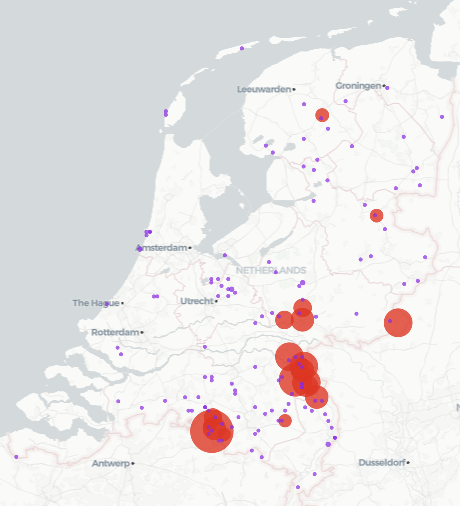
\includegraphics[width=\textwidth]{figures/Wildfires-April-2019-point.png}
\caption{Point-level geocoding results.}
\label{fig:wildfire-point-apr2019}
\end{subfigure}
\hfill
\begin{subfigure}[t]{0.49\textwidth}
\centering
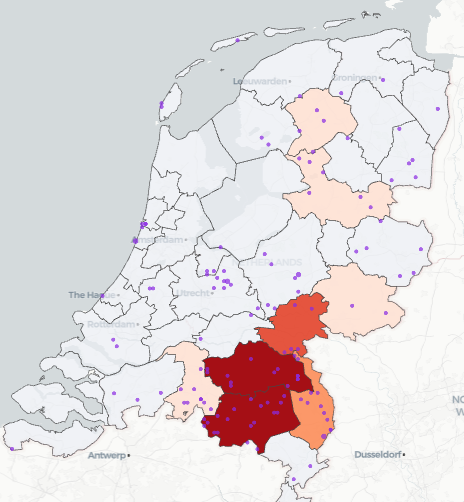
\includegraphics[width=\textwidth]{figures/Wildfires-April-2019-Nuts.png}
\caption{NUTS-3 aggregated geocoding results.}
\label{fig:wildfire-nuts-apr2019}
\end{subfigure}
\caption{Comparison of wildfire event locations extracted from news articles for April 2019 using point-level geocoding and NUTS-3 aggregation.}
\label{fig:wildfire-geocoding-comparison-apr2019}
\end{figure}

Similar to July 2018, Utrecht is underrepresented in the extracted dataset compared with the reference dataset. However, the overall spatial agreement remains strong, suggesting that newspaper-based wildfire extraction can capture regional wildfire patterns despite differences in reporting.

\paragraph{July 2019}

July 2019 shows the largest difference between the extracted wildfire events and the reference dataset. While the reference dataset contains many wildfire occurrences, only one newspaper-derived wildfire event was identified (Figure~\ref{fig:wildfire-geocoding-comparison-jul2019}).

\begin{figure}[!htbp]
\centering
\begin{subfigure}[t]{0.49\textwidth}
\centering
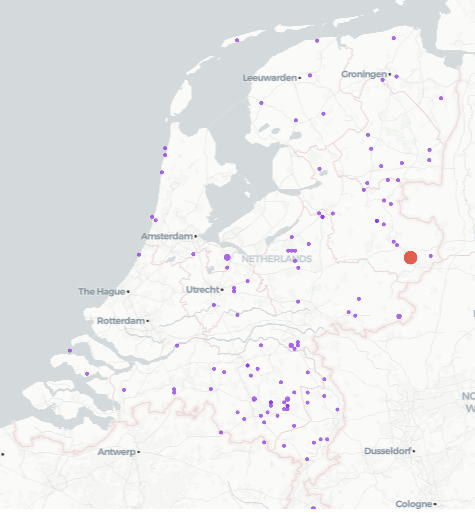
\includegraphics[width=\textwidth]{figures/Wildfires-July-2019-point.png}
\caption{Point-level geocoding results.}
\label{fig:wildfire-point-jul2019}
\end{subfigure}
\hfill
\begin{subfigure}[t]{0.49\textwidth}
\centering
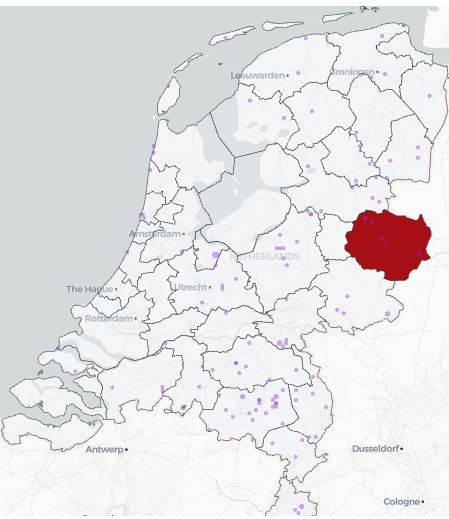
\includegraphics[width=\textwidth]{figures/Wildfires-July-2019-Nuts2.png}
\caption{NUTS-3 aggregated geocoding results.}
\label{fig:wildfire-nuts-jul2019}
\end{subfigure}
\caption{Comparison of wildfire event locations extracted from news articles for July 2019 using point-level geocoding and NUTS-3 aggregation.}
\label{fig:wildfire-geocoding-comparison-jul2019}
\end{figure}

Manual inspection showed that this article described a police investigation into suspected arson rather than a drought-related wildfire. Therefore, no direct drought-related wildfire impacts were extracted from the newspaper archive during this period. Since many drought-related articles were published during July 2019, this difference is unlikely to be caused by missing data collection.

One possible explanation is that newspapers do not report all wildfire occurrences. Fire department records may contain many small or local fires that are not considered important enough for news coverage. Therefore, the extracted dataset may represent reported wildfire impacts rather than all wildfire occurrences.

To investigate this limitation, the extraction was repeated while including both wildfire occurrence events and wildfire risk increase indicators. As shown in Figure~\ref{fig:graph-multiwildfire-risk-increase} and Figure~\ref{fig:wildfirerisk-increase-map}, the expanded dataset shows much closer agreement with the reference dataset.

\begin{figure}[!htbp]
    \centering
    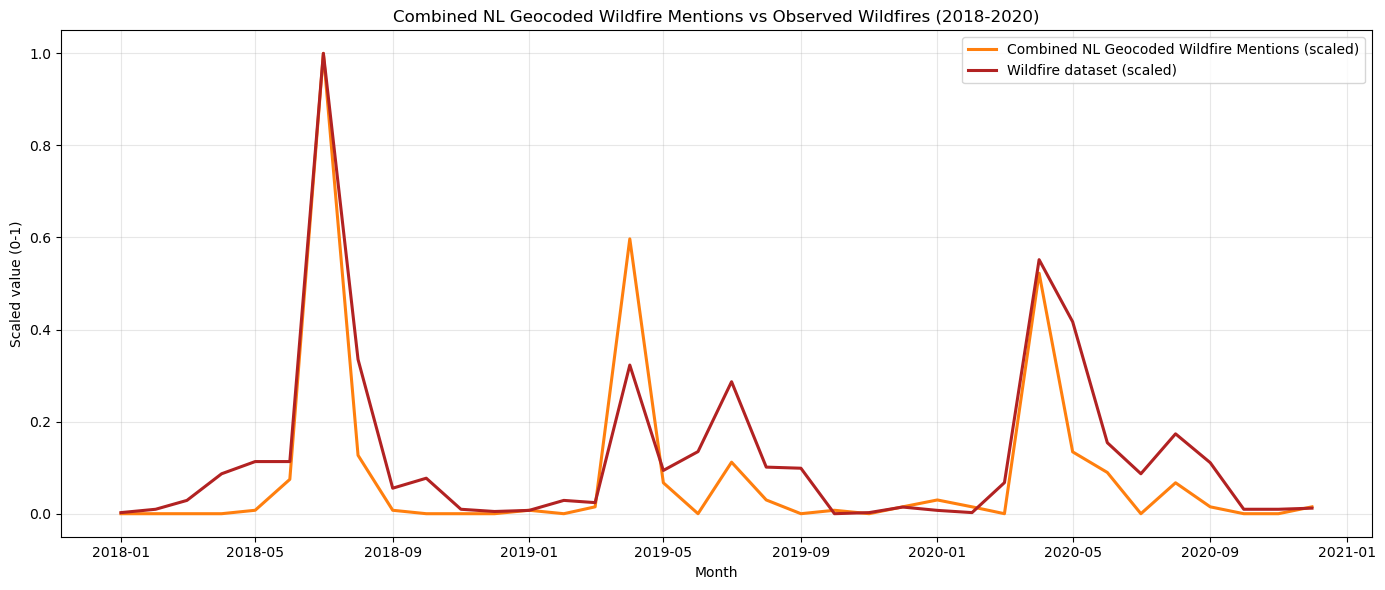
\includegraphics[width=0.75\linewidth]{figures/Wildfires-wildfire-risk increase.png}
    \caption{Normalized temporal comparison incorporating expanded wildfire risk indicators for July 2019.}
    \label{fig:graph-multiwildfire-risk-increase}
\end{figure}

\begin{figure}[!htbp]
    \centering
    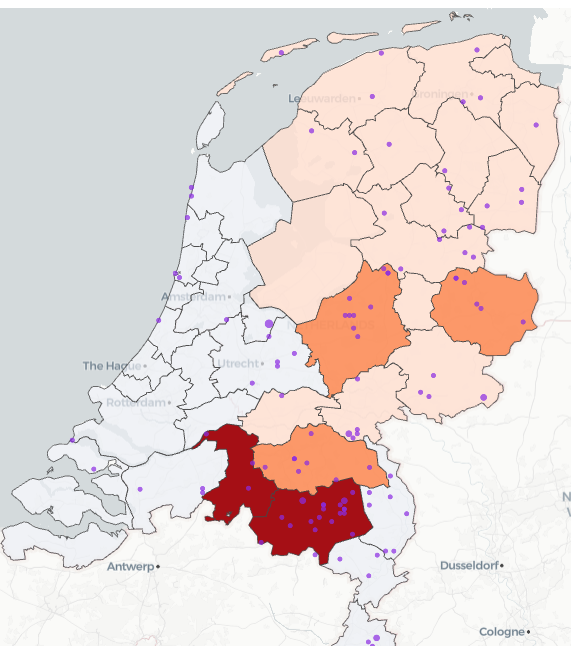
\includegraphics[width=0.30\linewidth]{figures/Wildfires-risk-increase-July-2019-nuts2.png}
    \caption{Spatial distribution of combined wildfire events and institutional risk warnings at the NUTS-3 level for July 2019.}
    \label{fig:wildfirerisk-increase-map}
\end{figure}

This indicates that newspaper-derived drought impact data can capture a broader wildfire-related signal, including periods of increased wildfire risk reported in newspapers, rather than only confirmed wildfire occurrences. This provides partial validation for the wildfire risk increase drought impact variable. It also demonstrates that there is a threshold before wildfire impacts are reported in newspapers compared with the reference dataset. Another hypothesis for this sudden mismatch in the data is that this was the second wildfire wave of the year and occurred during the summer holiday period. As a result, there may have been fewer journalists available to report on these events, leading to lower newspaper coverage despite wildfires occurring.



\subsection{Discussion of Spatial Reporting Differences}

In the previous section, we mentioned that fewer wildfires were observed in the Utrecht area during July 2018 in Fig. \ref{fig:wildfire-nuts-jul2018}.

After consulting with Femke Schasfoort, an expert on drought impacts in the Netherlands, we formulated several hypotheses to explain why substantially fewer wildfire impacts were identified in the Utrecht region during July 2018 and April 2019 compared to the reference dataset. An initial hypothesis was that the differences could be explained by soil type, as sandy soils are generally more vulnerable to wildfires. In Figure~\ref{fig:soil-type}, the Utrecht region appears to be predominantly covered by clay soils and therefore seems less vulnerable to wildfires. However, upon closer inspection, we found that the area within Utrecht where most wildfire impacts occurred in the reference dataset is actually located on sandy soils. This observation rejects the soil type hypothesis.

Another hypothesis relates to the reporting threshold discussed in the previous subsection. We concluded that wildfires likely need to exceed a certain threshold before they are reported in newspapers. It is possible that the wildfires occurring in the Utrecht region were relatively small or were effectively contained through government policies and efficient fire department responses. As a result, these events may never have reached the threshold required to be considered newsworthy, despite being included in the reference dataset. This explanation can be referred to as the reporting bias hypothesis or the rapid government response hypothesis. 

Overall, we observe clear correlations between the reference dataset, which records reported wildfire's, from any severity wildfires, and our impact dataset, which captures wildfires reported in newspaper articles. This indicates that both datasets have validity. However, the datasets do not match one-to-one due to reporting thresholds that need to be surpassed before wildfire events are reported in newspapers.




\label{sec:spatial-differences}

\begin{figure}[htbp!]
\centering
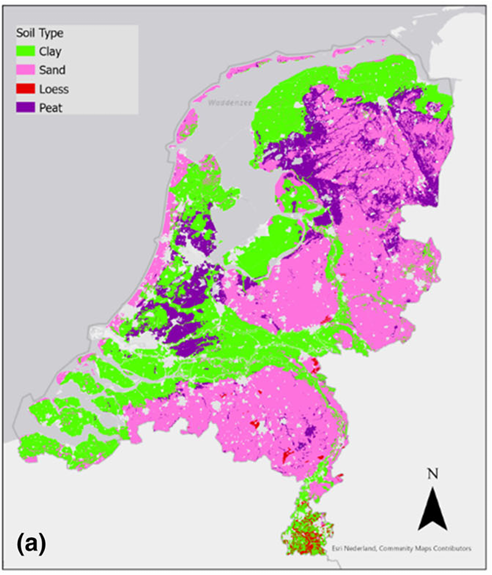
\includegraphics[width=0.5\linewidth]{figures/Soil map bron basisregistratie ondergrond.png}
\caption{National soil classification map of the Netherlands, sourced from the Basisregistratie Ondergrond (BRO).}
\label{fig:soil-type}
\end{figure}

